\documentclass[a4paper, 12 pt]{article}

\usepackage{amsfonts}
\usepackage{amsmath}
\usepackage{amsthm}
\usepackage{appendix}
\usepackage{bm}
\usepackage{booktabs}
\usepackage[usenames, dvipsnames]{color}
\usepackage{graphicx}
\usepackage{epstopdf}
\epstopdfsetup{update}
\usepackage{helvet}
\usepackage{hyperref}
\usepackage{indentfirst}
\usepackage{lscape}
\usepackage{morefloats}
\usepackage{natbib} \bibliographystyle{ecta}
%\bibliographystyle{abbrvnat}\bibpunct{(}{)}{;}{a}{,}{,}
\usepackage{setspace}
\usepackage{subcaption}
\usepackage[capposition=top]{floatrow}
\usepackage{subfloat}
\usepackage[latin1]{inputenc}
\usepackage{tikz}
%\usepackage[pdf]{pstricks}

\usetikzlibrary{trees}
\usetikzlibrary{decorations.markings}


\theoremstyle{plain}
\newtheorem{thm}{Theorem}
\newtheorem{cor}{Corollary}
\newtheorem{lem}[thm]{Lemma}
\newtheorem{proposition}{Proposition}
\newtheorem{assumption}{Assumption}
\newtheorem{definition}{Definition}

%MARGINS
 \topmargin   =  0.0in
 \headheight  =  -0.3in
 \headsep     =  0.7in
 \oddsidemargin= 0.0in
 \evensidemargin=0.0in
 \textheight  =  9.0in
 \textwidth   =  6.45in
% \setlength{\parindent}{4em}
 \setlength{\parskip}{1em}

\newcommand{\fmt}{.eps}
%\newcommand{\fmt}{.png}
\hypersetup{
    colorlinks=true,
    linkcolor=BlueViolet,
    citecolor=BlueViolet,
    filecolor=BlueViolet,
    urlcolor=BlueViolet
}




\setcounter{page}{0}
\begin{document}



\title{\Large{\textsc{Choosing Season of Birth}}\thanks{\scriptsize{We thank seminar participants at University of Surrey, participants in the ``Family Economics'' Workshop (Barcelona Graduate School of Economics) 2015, the Alicante Health Economics Workshop 2015, and the Vienna LHEDC Workshop 2015 for helpful comments and suggestions. Any errors contained in the paper are our own.}}}
\author{\small{Damian Clarke} \\ \small{University of Santiago de Chile} \and \small{Sonia Oreffice} \\ \small{University of Surrey \& IZA}  \and \small{Climent Quintana-Domeque} \\ \small{University of Oxford \& IZA}}

\date{{\small March 2016} \\ \vspace{2mm} \small{\textbf{Preliminary Draft}}}


%\author{Damian Clarke  \and Sonia Oreffice  \and Climent Quintana-Domeque  }
%\author{Damian Clarke \\ University of Oxford \and Sonia Oreffice \\ University of Surrey and IZA \and Climent Quintana-Domeque \\University of Oxford and IZA}


\maketitle
\thispagestyle{empty}

\begin{abstract}
We study the determinants of season of birth of the first child, for White non-Hispanic married women aged 25-45 in the US, using birth certificate and Census data. The prevalence of good season (quarters 2 and 3) is significantly related to mother's age, education, and smoking status during pregnancy. Moreover, those who do \emph{not} undergo assisted reproductive technology procedures present a higher prevalence of good season births. The frequency of good season is also higher and more strongly related to mother's age in states where cold weather is more severe, and varies with mother's occupation, exhibiting a particularly strong positive association with working in ``education, training, library''. All this evidence points to season of birth being a choice variable. In addition, season of birth determinants explain (at least) 10\% of the average difference in birth weights among first-born babies. Finally, we estimate the compensating wage differential for \emph{mothers} who work in \emph{non-education-related} jobs, which allows us to provide an upper-bound to the value of season of birth of about USD 2,600,000.
\end{abstract}
\emph{JEL Classification Codes}: I10, J01, J13.\\
\emph{Keywords}: quarter of birth, fertility timing, compensating wage differentials, birth outcomes.


\newpage
%\begin{spacing}{1.4}
\begin{doublespace}

%-------------------------------------------------------------------------------
\section{Introduction}
\paragraph{Motivation.} While the relevance of season of birth has been acknowledged at least since \citeauthor{Huntington38}'s \citeyear{Huntington38} book ``Season of Birth: Its Relation to Human Abilities'', it was not until the seminal article by \citet{AK1991}---in which quarter of birth was shown to be related to education and earnings in the USA---that season of birth became popular in economic research.\footnote{The validity of this approach has been questioned as quarter of birth is only weakly correlated with schooling. Even a weak correlation between quarter of birth and unobserved ability, for instance due to seasonal effects, might yield a large inconsistency in the IV estimates (\citealp{bound1995problems}). These validity concerns appear to be unsettled. For instance, a recent study shows that ``winter babies'' are more likely to have unmarried mothers, teenage mothers or less educated mothers, and that maternal schooling peaks for mothers who give birth in the second quarter (\citealp{BucklesHungerman2013}). However, these patterns in family background ``cannot account for the seasonal pattern in schooling and wages both of which exhibit third and fourth quarter peaks'' (\citealp{angrist2014mastering}).}  Recent work has unveiled a variety of channels, beyond school cutoff laws, through which season of birth may affect adult outcomes, for example, its potential effects on birth outcomes. Indeed, a clear and consistent pattern of ``good'' and ``bad'' seasons has emerged. In the US, winter months are associated with lower birth weight, education and earnings, while Spring and Summer are found to be ``good'' seasons (e.g., \citealp{BucklesHungerman2013}; \citealp{CS2013}). However, as yet, no study has considered season of birth as a choice outcome.  In this paper we examine this premise.  We consider if season of birth is itself a choice variable in a mother's childbearing decision, we investigate how a rich set of maternal characteristics are related to the prevalence of good season of birth, and provide an estimate of the value of the good season of birth.

\paragraph{Stylized facts.} We begin by documenting a set of rich and consistent stylised facts which suggest that season of birth is indeed a choice variable.  A significant ``good season'' gradient is observed by mother's age, by geographic variation in the climatic harshness of winter, by women's education and her occupation.  These relationships hold conditional on competing explanations such as non-random fetal death and non-random gestational length by age, geographic location, and educational attainment, and hold in varying contexts in the Southern and Northern Hemisphere.  We turn to the discussion of these stylised facts in the body of the paper.


\begin{figure}[htpb!]
\begin{center}
  \centering
  \caption{Prevalence of Good Season by Age}
  \includegraphics[scale=0.72]{./../results/nvss/graphs/goodSeasonAge.eps}
  \label{fig:goodByAge}
\end{center}
\vspace{-5mm}
\floatfoot{\textsc{Notes to figure \ref{fig:goodByAge}}: Coefficients and
standard errors are estimated by regressing ``good season'' on dummies
of maternal age.  Age groups 40-45 are omitted as the base group.  The full
sample consists of mothers aged 20-45.  For the omitted group, proportion
good season (and standard error) is 0.497(0.001).}
\end{figure}


\textbf{NOTE: This Figure should start at age 20!}

Figure \ref{fig:goodByAge} highlights the seasonality gap by age group: it plots the frequency of good season for each age, compared to the omitted base group of 40-45 year olds.  Two features are worth mentioning. First, there is a decreasing gap in age from 25 to 45. In particular, the relative prevalence of good season is highest (more than 3 pp) for mothers aged 25-34, while it is essentially zero for mothers aged 40-45. Second, the relationship between seasonality gap and age is non-monotonic: The gap increases as women approach the age of 28, is approximately flat up until the age of 31, and then follows a downward trajectory for women aged 32-39. While the former feature is consistent with biological constraints whereby younger women can better control their fertility and optimally time their births, the latter suggests that the prevalence of good season of birth cannot be entirely accounted for by the higher biological ability of young mothers to engage in optimal planning.


\begin{table}[htpb!]\caption{Percent of Births (NVSS 2005-2013)}
\label{bqTab:singleSum}\begin{center}\begin{tabular}{lcccccc}
\toprule \toprule
& \multicolumn{4}{c}{Seasons} & \multicolumn{2}{c}{Characteristics} \\ \cmidrule(r){2-5} \cmidrule(r){6-7}
& Bad    & Good   & Diff. & Ratio & $< $37 & ART \\
& Season & Season &       &       & Gestation  & \\
&     &   &       &       & Weeks  &     \\\midrule\multicolumn{5}{l}{\textsc{Panel A: By Age}}\\
\begin{footnotesize}\end{footnotesize}&
\begin{footnotesize}\end{footnotesize}&
\begin{footnotesize}\end{footnotesize}&
\begin{footnotesize}\end{footnotesize}&
\begin{footnotesize}\end{footnotesize}\\
20-24 Years Old&48.41&51.59&3.18&1.07&0.08&0.00
\\
25-27 Years Old&47.94&52.06&4.12&1.09&0.08&0.00
\\
28-31 Years Old&47.77&52.23&4.46&1.09&0.08&0.01
\\
32-39 Years Old&48.69&51.31&2.62&1.05&0.09&0.02
\\
40-45 Years Old&49.89&50.11&0.22&1.00&0.12&0.08
\\
 &&&&&& \\\multicolumn{7}{l}{\textsc{Panel B: By Education}}\\
\begin{footnotesize}\end{footnotesize}&
\begin{footnotesize}\end{footnotesize}&
\begin{footnotesize}\end{footnotesize}&
\begin{footnotesize}\end{footnotesize}&
\begin{footnotesize}\end{footnotesize}\\
No College&49.07&50.93&1.86&1.04&0.10&0.00
\\
Some College +&48.07&51.93&3.86&1.08&0.08&0.01
\\
 &&&&&& \\
\midrule\multicolumn{7}{p{11.8cm}}{\begin{footnotesize}\textsc{Notes:} Sample consists of all first-born, singleton children born to white, non-hispanic \textbf{married} mothers aged between 20-45 for whom     education and smoking during pregnancy are available. Good season refers to birth quarters 2 and 3 (Apr-Jun and Jul-Sept).  Bad season refers to quarters 1 and 4 (Jan-Mar and Oct-Dec). ART refers to the proportion of  women who undertook assisted reproductive technologies that resulted in these births.
\end{footnotesize}} \\ \bottomrule
 \end{tabular}\end{center}\end{table}


The patterns in Figure 1 are summarized in Table 1, which contains information on the percent of births by good season, but also on prematurity and use of ART. These percentages are examined by age and education groups. Good season is non-monotonically related to age: it is 51.59\% among younger women (aged 20-24), it increases to 52.23\% among women aged 28-31, and it decreases to 50.11\% among older women (aged 40-45). These non-monotonic relationship can reflect two opposing effects: a selection effect --very young mothers tend to be negatively selected-- and a biological effect --older mothers have less control on their fertility timing than younger ones. The positive relationship between good season and age from 20 to 31 could capture a (positive) net selection effect, while the negative relationship between good season and age from 31 to 45 could capture a (negative) net biological effect.%\footnote{The same type of investigation is developed with Spanish birth certificate data for the years 2007-2013 in a country with a much more generous maternity leave environment than the US. That is, this allows us to strengthen our interpretation of the choice nature of season of birth and to examine its relationship with mothers' labor force participation and occupation, information that is not at all recorded in the US certificates.}

With regards to education, more educated women are more likely to hit the good season. Looking at the \% of premature newborns (born within 37 weeks of gestation) and those from women undertaking ART, we find that prematurity increases with age, from 8\% among 20-24 years old to 12\% for women aged 40-45, as does ART, from 1\% among 28-31 years old to 8\% among women aged 40-45. First, newborns of women without a college degree are more likely to be premature than those of their counterparts (10\% vs. 8\%), and among high-educated women the \% of newborns is higher than among their counterparts (1\% vs. 0\%). Whether higher education reflects better information regarding the benefits of good season or higher education correlates with higher ``job flexibility'' to hit the good season is an open question that we postpone to our analysis with ACS data.

Given the prominence of fertility planning in balancing people's work and family life as well as the above stylized facts, it is hard to believe that season of birth may simply be a matter of chance. In addition, far from assuming that the average woman is aware that birth weight and the child's future earnings are affected by birth timing, it is sufficient to consider that the average woman has a sense that, on the one hand, winter months may be tougher birth months because of cold weather and higher disease prevalence,\footnote{According to the \citet{CDC2014}, from 1982-83 through 2013-14, the ``peak month of flu activity'' (the month with the highest percentage of respiratory specimens testing positive for influenza virus infection), has been February (14 seasons), followed by December (6 seasons) and January and March (5 seasons each): \href{http://www.cdc.gov/flu/about/season/flu-season.htm}{http://www.cdc.gov/flu/about/season/flu-season.htm}} and on the other, work commitments make it much easier to take time off with a Spring-Summer birth.\footnote{The report on fertility, family Planning, and women's health (\citealp{CDC1997}) notes that some women do not take maternity leave due to the timing birth relative to their job schedules, and gives the example of school teachers who deliver during summer break.}
%We examine these motivations and women's \emph{stated choices} in a complementary survey to support the extensive set of stylised facts observed in birth and labour market data.
To examine the value of good season of birth, we estimate the value of season of birth using a standard compensating differential framework, that is, comparing the earnings of mothers in non-teacher occupations and those of their counterparts.

\paragraph{This paper.} We first present novel correlates of season of birth, investigating women's decision of when to have their first birth in terms of season of birth, for White non-Hispanic married women aged 25-45. Using US Vital Statistics data from 2005 to 2013 on all first singleton births, we show that the prevalence of good season (quarters 2 and 3) is very significantly related to mother's age and education. In addition, we find that women who do \emph{not} undergo assisted reproductive technology (ART) are 3 percentage points more likely to give birth in the good season. This finding, which is robust to controlling for gestation length fixed effects, is consistent with season of birth being a choice outcome, if undergoing ART is associated to \emph{no} longer being under control of birth timing. Moreover, if women undergoing ART cannot choose season of birth, we should expect to find no seasonality gap, and we present supportive evidence for this prediction. We then examine how birth outcomes, such as birth weight, prematurity ($<37$ weeks of gestation) and APGAR scores, are related to season of birth controlling for mother's characteristics. We find that being born in the good season is positively associated to better birth outcomes.

We then examine data on all births occurring in the American Community Survey (ACS) from 2005-2014.  Along with season of birth and mother's characteristics, the ACS data allow us to examine the interaction of a child's season of birth with his mother's labour market decisions.  We find important interactions with labour market choices: in professions in which strong seasonality of work hours exist (such as educators), mothers are additionally more likely to choose good season of birth, and this holds conditional on observed age, education, and weather patterns.

%Finally, we document that this result is not unique to the United States and its particular institutional and labour market context.  Using vital statistics from Spain we find that similar gradients in good season exist by age of mothers, by temperature, and by job type.  Once again, these findings are consistent with choice, as we can rule out that it is driven by selective fetal death or selective birth prematurity.

%In the second part of our investigation, we conduct our own survey to elicit information on the choices which women make (or are believed to make), and the degree to which beliefs about the benefits of good season affect those choices.  We recruit a pool of online survey respondents from Amazon's Mechanical Turk\footnote{Mechanical Turk (or MTurk) is a service provided by Amazon which allows for the recrutiment of a pool of workers to respond to a survey or perform other online tasks for payment.  The use of MTurk in experimental research is growing.  For further discussion, see for example \citet{Berinskyetal2012}.}, and ask respondents about their beliefs and choices.  This survey is currently being implemented, and will provide additional information to complement observational results from the US and Spanish vital statistical results, and the US survey data described above.


\paragraph{Related literature.} While \citet{CS2013} explain the first quarter of birth disadvantage through the negative impact of the disease environment on birth weight and gestational weeks in cold months, \citet{BucklesHungerman2013} emphasize the role of maternal characteristics in shaping the later socioeconomic disadvantage of winter-born individuals, showing that the mothers of those children are significantly less educated, less likely to be married or white, and more likely to be teenagers.\footnote{\citet{AlbaCaceres2014} describe similar findings for Chile and Spain.} Recent work by \citet{Barrecaetal2015} suggests that individuals may make short shifts in conception month in response to very hot days, with resulting declines and rebounds in following months.

Apart from the work by \citet{BucklesHungerman2013}, which may suggest the possibility that season of birth is \emph{not} random, and \citet{Barrecaetal2015}'s work on temperature and short-term shifts, there is a literature on ``exact'' birth timing analyzing the joint decision of parents and physicians to alter the delivery of an already existing pregnancy (in response to non-medical incentives). \citet{Shigeoka2015}, focusing on the distribution of births between December and January,  finds that in Japan many births are shifted one week forward around the school entry cutoff date. \citet{DCChandra1999} and \citet{LaLumiaetal2015} report that in the US parents may move expected January births backwards to December to gain tax benefits, while in Australia \citet{GansLeigh2009} estimate that parents moved forward June deliveries to become eligible for a newly introduced ``baby bonus''. Fewer births are documented on holidays \citep{Rindfuss1979} and weekends \citep{Gould2003}, less auspicious dates \citep{Almond15} or on medical professional meeting dates \citep{GLV2007}. 

Although this body of evidence clearly shows that parents may be willing and able to manipulate birth timing, it represents a choice made well after conception occurs. To the best of our knowledge, ours is the first economic analysis of the planning of season of birth.

\paragraph{Structure of the paper.} Section \ref{scn:data} describes the data sources. Section \ref{scn:results} presents the analysis of the correlates of season of birth. Section 4 provides a simple framework and estimates the ``value'' of good season of birth. Section 5 presents the analysis of how birth outcomes correlate with season of birth controlling for mothers' characteristics. Section 6 concludes the paper.

\newpage
%-------------------------------------------------------------------------------
\section{Data Sources and Descriptive Statistics}
\label{scn:data}
\subsection{Birth Certificate Data}
\label{bqSscn:USAdata}
Data on all births occurring each year in the United States are collected from birth certificate records, and publicly released as the National Vital Statistics System (NVSS) by the National Center of Health Statistics. These data are available for all years between 1968 and 2013, with all registered births in all states and the District of Columbia reported from 1984 onwards.\footnote{Prior to 1984, a 50\% sample was released for those states that did not submit their birth records on electronic, machine readable tape \citep{Martinetal2015}.}  In total, more than 99\% of births occurring in the country are registered \citep{Martinetal2015}. The birth certificate data record important information on births and their mothers. For the mother, this includes age, race, ethnicity, marital status, education, smoking status during pregnancy, and since 2009 assisted reproductive technology (ART) use. For the newborn, in addition to place and time of birth, measures include birth parity, singleton or multiple births status, gestational length (in weeks), birth weight, and one- and five-minute APGAR scores.\footnote{Birth certificates have gone through two important revisions in the variables reported: one in 1989 and the other in 2003.  These revisions (described fully in \citealp{NCHS2000}) were implemented by states at different points in time.  Prior to 2005, all states had fully incorporated the 1989 revision.  In the most recent wave of birth certificate data (2013), 41 states, containing 90.2\% of all births, had switched to the more recent 2003 revision.  Importantly, the revised data include a different measure of education, a wider range of birth outcomes, and do not include the mother's smoking status. ART use information was first released in 2009. These changes mean that we do not have information for all variables over the whole period of analysis.} %\footnote{Complete details of missing variables are available in Table \ref{bqTab:SumStatsNVSS}, and further details regarding birth certificate revisions and the effect on reported variables and representativeness of the country as a whole are provided in appendix \ref{bqScn:datApp}.}
%As such, our principal estimation sample is restricted only to those women for whom all covariates are recorded.


Our estimation sample consists of birth years 2005-2013, and we retain all singleton first-births to White, non-Hispanic married mothers aged 25-45 who are issued an updated birth certificate with available education and smoking status.\footnote{The analysis is replicated including unmarried women in the online appendix to this paper.} We focus on first births, given that higher-order births also involve the additional decision of birth spacing and the role of experience, possibly underestimating the determinants of the choice of season of birth if planning improves with higher-order pregnancies. In the same vein, we consider only singleton births.\footnote{ Analyses using second-births and twin birth data are provided in the appendix.} This results in a sample of 2,260,745 births, 2,259,553 of which have gestation length recorded, that is, for whom conception month is known.


%-------------------------------------------------------------------------------
\subsection{Mother's Occupation Data}
Unfortunately the US birth certificate data do not contain information on mother's occupation. In order to investigate the role of mother's occupation in explaining season of birth we supplement our analysis of NVSS data with the American Community Survey (ACS) conducted by the United States Census Bureau on a representative 1\% of the US population every year.\footnote{ Given that Census data do not provide gestational length, season of birth is defined as the actual quarter of birth, not the expected one.} Along with demographic and socioeconomic details on women, we observe their labor market outcomes, and specifically occupation which is coded using the standard Census occupation codes and defined as the occupation in your current job or in the job you had in the previous 5 years. We use data from 2005 to 2014, the most recent available survey, and focus on White non-Hispanic married women aged 25-45 who are either head of the household or spouse of the head of the household, who have a first singleton child who is at most one year old.\footnote{We exclude women who are in the military, in a farm household, or currently in school.}

We use the ACS data in two instances: the first to study the relationship between season of birth of first-born and occupation; the second to study the relationship between earnings and job type, and their different relationship for mothers and non-mothers. For the former analysis, we retain only women who were employed in the previous 5 years in non-military occupations where each occupation must have at least 500 women over the entire range of survey years, while for the latter, we add to our previous sample women without children and women with more than one child.\footnote{ The handful of observations of households containing two women have been excluded.}


%-------------------------------------------------------------------------------
\subsection{Temperature and Unemployment Data}
Temperature data are provided by the National Centers for Environmental Information from 1895 onwards, updated monthly. We collate measures of monthly means, maxima and minima for each state, year and month over our time period of analysis, as described in \citet{Voseetal2014}. These are available for all states with the exception of Hawaii and the District of Columbia (DC). We assign births that take place in DC the temperature data from Maryland, a contiguous state.

Unemployment data at the level of the state, year and month is created from the Bureau of Labor Statistics' (BLS) online monthly time series
data.\footnote{Full records are available at \href{http://download.bls.gov/pub/time.series/la}{http://download.bls.gov/pub/time.series/la}.} These data come from the Local
Area Unemployment Statistics (LAUS) Series, and are available for all states plus DC for the entire time period of interest. Measures of temperature and unemployment are calculated at the year by month and state level, and are merged by conception (not birth) month.  We are able to calculate both conception and birth month, given that gestation is reported in the birth data.




%-------------------------------------------------------------------------------
\subsection{Descriptive Statistics}


Table \ref{bqTab:SumStatsMain} presents the summary statistics. The first panel of the table shows that women are on average 30 years old, and 97\% are aged below 40 by the time of their first birth (``younger''). For those birth certificates with available mother's education and smoking information, 77\% have at least some college education; for those with non-missing smoking information, 3\% reported having smoked during pregnancy. Finally, for the five most recent years in our sample (2009-2013), we have information on the use of ART procedures: 1\% of these first-births were achieved through ART.

In the second panel, we present detailed information on birth outcomes. 52\% of babies to first-time, married mothers are born in the good season, defined as quarters 2 and 3; taking into account gestational length, a similar proportion (52\%) of the newborns were planned for the good season. It is noteworthy that in the US none of the public holidays falls any close to the frontiers between the good and bad seasons defined above\footnote{Nationally Observed Public Holidays are: New Year's Day, Martin Luther King Jr. Day, Presidents' Day, Memorial Day, July 4, Labor Day, Columbus Day, Veteran's Day, Thanksgiving, Christmas Day.}. Regarding gender, 49\% are girls. Finally, we have information on birth ``quality'' measures, including birth weight, prematurity ($<37$ weeks of gestation) and APGAR score. The averages of these measures (3,353 grams, 8\%, 8.8, respectively) are consistent with those from previous studies.

%Table \ref{bqTab:singleSum} investigates the seasonality of birth by mother's age in binary age groups, and education (no college vs. at least some college). Panel A shows that young women (aged 28-31) are 4.5 percentage points (pp) more likely to give birth in the good season than in the bad season (52.2\% good vs. 47.8\% bad), whereas for older women the odds are virtually 50-50 (50.1\% good vs. 49.9\% bad). In Panel B we also observe that more educated women have a higher probability of giving birth in the good season (51.9\% vs. 48.1\%), while the gap for less educated women is 1.9 pp (50.9\% vs. 49.1\%).\footnote{The same type of investigation is developed with Spanish birth certificate data for the years 2007-2013 in a country with a much more generous maternity leave environment than the US. That is, this allows us to strengthen our interpretation of the choice nature of season of birth and to examine its relationship with mothers' labor force participation and occupation, information that is not at all recorded in the US certificates.} \textbf{Whether higher education reflects better information regarding the benefits of good season or higher education correlates with higher ``job flexibility'' to hit the good season is an open question that we postpone to our analysis with ACS data. }


\begin{table}[htpb!]
 \begin{center}
\caption{Descriptive Statistics (NVSS 2005-2013)}
 \label{bqTab:SumStatsMain}\begin{tabular}{lccccc}
 \toprule\toprule \vspace{5mm}
& N & Mean & Std. Dev. & Min. & Max. \\ \midrule
\multicolumn{6}{l}{\textbf{Panel A: Mother}} \\
Mother's Age        &     2260745&       30.28&        3.92&          25&          45\\
Young (aged 25-39)  &     2260745&        0.97&        0.16&           0&           1\\
Aged 25-27          &     2260745&        0.28&        0.45&           0&           1\\
Aged 28-31          &     2260745&        0.39&        0.49&           0&           1\\
Aged 32-39          &     2260745&        0.30&        0.46&           0&           1\\
Aged 40-45          &     2260745&        0.03&        0.16&           0&           1\\
Some College +&     2260745&        0.77&        0.42&           0&           1\\
Years of education  &     2260745&       15.59&        1.59&           4&          17\\
Smoked during Pregnancy&     2260745&        0.03&        0.18&           0&           1\\
Used ART (2009-2013 only)&     1572674&        0.01&        0.11&           0&           1\\

 \multicolumn{6}{l}{\textbf{Panel B: Child}}\\
 Good season of birth (birth date)&     2260745&        0.52&        0.50&           0&           1\\
Good season of birth (due date)&     2259553&        0.52&        0.50&           0&           1\\
Female              &     2260745&        0.49&        0.50&           0&           1\\
Birthweight (grams) &     2255282&     3352.85&      535.94&         500&        5000\\
Low Birth Weight ($<$2500 g)&     2255282&        0.05&        0.22&           0&           1\\
Weeks of Gestation  &     2259553&       39.02&        2.17&          17&          47\\
Premature ($<$ 37 weeks)&     2259553&        0.08&        0.27&           0&           1\\
APGAR (1-10)        &     2248425&        8.78&        0.82&           0&          10\\

\midrule\multicolumn{6}{p{14.2cm}}{\begin{footnotesize}\textsc{Notes:} Sample is identical to that described in table \ref{bqTab:singleSum}, however only for women aged 25-45.  This  is the main estimation sample.                                    \end{footnotesize}} \\ \bottomrule
 \end{tabular}\end{center}\end{table}



\newpage
%-------------------------------------------------------------------------------
\section{Season of Birth Correlates}
\label{scn:results}
\subsection{Mother's Age and ART usage}
We begin by examining the birth prevalence by month for two age groups of younger and older first time mothers (28-31 vs. 40-45). Figure \ref{bqFig:concepMonth} (a) shows that the gap between the two groups is positive precisely in the months representing the ``good'' season (April to September) and negative in the ``bad'' season (October to March). This finding is consistent with ``younger'' mothers being less biologically constrained than ``older'' mothers when making their fertility decision, \emph{ceteris paribus}. Good and bad seasons are defined as the \emph{expected} (intended) season of birth, which we compute from the actual month of birth, subtracting gestational length and adding nine months.\footnote{ Using actual or expected season of birth is immaterial for our findings.}

\begin{figure}[htpb!]
\begin{center}
\caption{Birth Prevalence by Month, Age Group, and ART Usage}
\label{bqFig:concepMonth}
\begin{subfigure}{.5\textwidth}
  \centering
  \includegraphics[scale=0.55]{./../results/nvss/graphs/conceptionMonth.eps}
  \caption{Proportion of Conceptions in Each Month}
  \label{fig:concepAbs}
\end{subfigure}%
\begin{subfigure}{.5\textwidth}
  \centering
  \includegraphics[scale=0.55]{./../results/nvss/graphs/conceptionMonthART.eps}
  \caption{Proportion of Conceptions (ART Only)}
  \label{fig:concepAbsART}
\end{subfigure}
\end{center}
\floatfoot{\textsc{Notes to figure \ref{bqFig:concepMonth}}: Month of conception
is calculated by subtracting the rounded number of gestation months (gestation in
weeks $\times$ 7/30.5) from month of birth.  Each line presents the proportion of
all births conceived in each month for the relevant age group.}
\end{figure}

If women undergoing ART to achieve their first birth cannot and do \emph{not} choose season of birth, we should expect to find no seasonality gap in their births: that is exactly what the patterns in Figure \ref{bqFig:concepMonth} (b) show.\footnote{Note that the fraction of ART babies for women aged 28-31 is 1\%, while for mothers younger than 28 the percentage decreases to 0\%.} Moreover, when examining the distribution of ART births over the year, the entire difference in the proportion of good season births appears to be driven by a large reduction of ART conceptions occurring in December. This is in line with the seasonality of treatment availability of ART clinics, which in many cases do not offer complex fertility treatments such as IVF (in vitro fertilization) in December due to Christmas closure and the daily attention and last minute changes that these treatments require.\footnote{ This is supported by anecdotal evidence on fertility clinics operations.} When the choice of season of birth is not in women's hands, we observe no seasonality at all.

In Table \ref{tab:bqMain} we investigate the determinants of good season of birth. In column 1 we see that ``younger'' women are approximately 2 pp more likely to have their first child in the good season than ``older'' women (aged 40-45). These age dummies reflect the graphical pattern observed in Figure 1 of a non-monotonic relationship between age and good season with a peak good season age of 28 years, and mirror the descriptive statistics in Table 1. This difference is robust to the following additional control variables: state and year fixed effects, education (an indicator for having some college or above), and (an indicator for) smoking during pregnancy (columns 2-4). In addition, high-educated women are between 0.7 and 1 percentage points more likely to have their first born child in the good season than their counterparts, which is only half of the difference between younger and older women. Women who smoked during pregnancy are 1.2 percentage points less likely to ``hit'' the good season. %Hence, a mother's age seems to be the most relevant driving force behind season of birth.
Finally, in columns 5-7, we investigate the role of undergoing an ART procedure. Since this information is available only from 2009 to 2013, we replicate column 4 with this restricted sample in column 5, finding the same results. In column 6 we include an ART indicator (1 if the birth did not happen through an ART procedure, 0 otherwise), and estimate a strongly positive significant coefficient: Women who underwent ART are about 3 pp less likely to give birth in the good season. This finding, which is robust to controlling for gestation length fixed effects, is consistent with season of birth being a choice variable, if undergoing ART is associated to no longer being under control of (or not caring about) birth timing.

\vspace{10mm}

\begin{table}[htbp]\centering
\def\sym#1{\ifmmode^{#1}\else\(^{#1}\)\fi}
\caption{Season of Birth Correlates  \label{tab:bqMain}}
\begin{tabular}{l*{5}{c}}
\toprule
                    &\multicolumn{1}{c}{(1)}   &\multicolumn{1}{c}{(2)}     &\multicolumn{1}{c}{(3)}   &\multicolumn{1}{c}{(4)}   &\multicolumn{1}{c}{(5)}   \\
                    & Good Season   & Good Season   &  Good Season   & Good Season   & Good Season   \\
\midrule
Aged 25-27          &       0.020***&       0.022***&       0.021***&       0.023***&       0.021***\\
                    &     [0.002]   &     [0.002]   &     [0.002]   &     [0.003]   &     [0.003]   \\
Aged 28-31          &       0.022***&       0.023***&       0.021***&       0.024***&       0.022***\\
                    &     [0.002]   &     [0.002]   &     [0.002]   &     [0.003]   &     [0.003]   \\
Aged 32-39          &       0.013***&       0.013***&       0.012***&       0.013***&       0.011***\\
                    &     [0.002]   &     [0.002]   &     [0.002]   &     [0.003]   &     [0.003]   \\
Some College +      &               &               &       0.009***&       0.007***&       0.008***\\
                    &               &               &     [0.001]   &     [0.001]   &     [0.001]   \\
Smoked in Pregnancy &               &               &      -0.012***&      -0.012***&      -0.012***\\
                    &               &               &     [0.002]   &     [0.002]   &     [0.002]   \\
Did not undergo ART &               &               &               &               &       0.027***\\
                    &               &               &               &               &     [0.004]   \\
Constant            &       0.501***&       0.499***&       0.503***&       0.550***&       0.527***\\
                    &     [0.002]   &     [0.002]   &     [0.062]   &     [0.077]   &     [0.077]   \\
\midrule
Observations        &     2259553   &     2259553   &     2259553   &     1571996   &     1571996   \\
F-test of Age Dummies&0.000&0.000 &0.000&0.000&0.000 \\
State and Year FE  &                &    Y          &                          Y  &      Y  &    Y\\ Gestation FE & &&Y&Y&Y\\
2009-2013 Only& &&&Y&Y\\ \bottomrule
\multicolumn{6}{p{15cm}}{\begin{footnotesize} Independent
variables are all binary
measures. F-test for age dummies refers to the p-value on the
test of equality of the three age dummies. Heteroscedasticity
robust standard errors are reported in parentheses.
***p-value$<$0.01, **p-value$<$0.05, *p-value$<$0.01.
\end{footnotesize}}\end{tabular}\end{table}

\vspace{10mm}
\vspace{10mm}

Table 4 shows that including fetal deaths (deaths occurring between 25 and 44 weeks of gestation) does not affect our findings.\footnote{ Accounting for fetal deaths is also a crude way to account for the influence of miscarriages, which we cannot observe.}

\begin{table}[htbp]\centering
\def\sym#1{\ifmmode^{#1}\else\(^{#1}\)\fi}
\caption{Season of Birth Correlates (Including Fetal Deaths) \label{tab:FDeaths}}
\begin{tabular}{l*{4}{c}}
\toprule
                    &\multicolumn{1}{c}{(1)}   &\multicolumn{1}{c}{(2)}   &\multicolumn{1}{c}{(3)}   &\multicolumn{1}{c}{(4)}   \\
                    & Good Season   & Good Season   & Good Season   & Good Season   \\
\midrule
Aged 25-27          &       0.020***&       0.022***&       0.022***&       0.021***\\
                    &     [0.002]   &     [0.002]   &     [0.002]   &     [0.002]   \\
Aged 28-31          &       0.022***&       0.023***&       0.023***&       0.022***\\
                    &     [0.002]   &     [0.002]   &     [0.002]   &     [0.002]   \\
Aged 32-39          &       0.013***&       0.013***&       0.013***&       0.012***\\
                    &     [0.002]   &     [0.002]   &     [0.002]   &     [0.002]   \\
Smoked in Pregnancy &               &               &      -0.015***&      -0.014***\\
                    &               &               &     [0.002]   &     [0.002]   \\
Constant            &       0.501***&       0.499***&       0.499***&       0.517***\\
                    &     [0.002]   &     [0.002]   &     [0.002]   &     [0.061]   \\
\midrule
Observations        &     2269645   &     2269645   &     2269645   &     2269645   \\
F-test of Age Dummies&0.000&0.000&0.000&0.000 \\
State and Year FE&&Y&Y&Y\\  Gestation FE &&&&Y \\ \bottomrule
\multicolumn{5}{p{14 cm}}{\begin{footnotesize} Main sample is
augmented to include fetal deaths occurring between 25 and 44
weeks of gestation. Fetal death files
include only a subset of the full set of variables included in the
birth files, so education and ART controls are not included. F-test
for age dummies refers to the p-value on the test of equality of
the three age dummies. Heteroscedasticity robust standard errors
are reported in parentheses.
***p-value$<$0.01, **p-value$<$0.05, *p-value$<$0.01.
\end{footnotesize}}\end{tabular}\end{table}


\subsection{Education, Smoking during Pregnancy and Selection}

%As we have shown in Figure \ref{bqFig:YoungvOld}, there is no seasonality gap among women using ART. In Table \ref{tab:ART2024} we perform an analysis including women aged 20-24, if only because women undergoing ART who are very young (20-24), well below the mean age of mother at first birth in the US (26 years in 2013; see \citealp{Martinetal2015}), are likely to suffer from serious infertility problems and may be those who end up in the bad season. While these results suggest that ART users are actually on average more likely to give birth during the ``bad season'', no systematic or statistically significant difference is observed when comparing older to younger women (figure \ref{fig:concepAbsART}).  Indeed, when examining the distribution of ART births over the year, the entire difference in the proportion of good season births appears to be driven by a large reduction of ART conceptions occurring in January.  This is in line with seasonality in opening hours of ART clinics, which in many cases have extended periods of closure in December.  This is supported by anecdotal evidence from an online search of clinic opening hours.


%Figure \ref{fig:mapYoung} reveals that, for ``younger'' women, good season is more prevalent in the North of the US than in the South. However, this pattern does not hold for ``older'' women, as we can see in Figure \ref{fig:mapOld}. Specifically, among ``younger'' women, a much higher proportion of good season births are observed in the northern states where the winter temperature is more severe. Interestingly, there is a North-South gradient, southern states with milder Winter exhibit lower proportion of births in good seasons. Strikingly, no such geographical pattern is observed of first births to ``older'' mothers, with the proportion of good season births appearing to be unrelated to geographic location of the state.

We argued that the non-monotonic relationship between good season of birth and age can reflect the influence of two opposing effects: a \emph{selection} effect --younger mothers tend to be negatively selected-- and a \emph{biological} effect --older mothers have less control on their fertility timing than younger ones. In Table 5 we add very young women (aged 20-24) to our main sample and find several interesting findings. First, very young women are 0.4 percentage points less likely to have their first child in the good season, and women using ART are 3 percentage points less likely to hit the good season. Controlling for state and year fixed effects decreases the relationship with age but it strengthens the correlation with ART usage. Interestingly, when controlling for smoking during pregnancy and mother's education, the negative relationship between being a young mother and good season disappears, while the ART correlation is robust to such adjustment: women who smoked during pregnancy are 1.3 percentage points less likely to have their first child in the good season, and educated women are about 1 percentage point more likely to hit the good season. This table reveals that the stylized fact that very young mothers are less likely to hit the good season captures negative selection: the younger mothers are less educated and more likely to smoke. Once these two factors are accounted for, these younger mothers are not less likely to hit the good season (actually, the coefficient in column 6 is positive), showing that the relationship between season of birth and age is not only governed by a mere biological mechanism, but there is a decision-making process behind. Moreover, we can also see that the ART correlation reflects a biological mechanism, since this relationship is robust to controlling for education and smoking during pregnancy.

\begin{table}[htbp]\centering
\def\sym#1{\ifmmode^{#1}\else\(^{#1}\)\fi}
\caption{Season of Birth Correlates: Very Young (20-24) and ART users\label{tab:ART2024}}
\begin{tabular}{l*{5}{c}}
\toprule
                    &\multicolumn{1}{c}{(1)}   &\multicolumn{1}{c}{(2)}   &\multicolumn{1}{c}{(3)}   &\multicolumn{1}{c}{(4)}   &\multicolumn{1}{c}{(5)}   \\
                    & Good Season   & Good Season   & Good Season   & Good Season   & Good Season   \\
\midrule
Aged 20-24          &      -0.004***&      -0.002** &      -0.002   &       0.000   &       0.001   \\
                    &     [0.001]   &     [0.001]   &     [0.001]   &     [0.001]   &     [0.001]   \\
Did not undergo ART &       0.030***&       0.033***&       0.033***&       0.033***&       0.033***\\
                    &     [0.003]   &     [0.003]   &     [0.003]   &     [0.003]   &     [0.003]   \\
Smoked in Pregnancy &               &               &      -0.013***&               &      -0.011***\\
                    &               &               &     [0.002]   &               &     [0.002]   \\
Some College +      &               &               &               &       0.010***&       0.009***\\
                    &               &               &               &     [0.001]   &     [0.001]   \\
Constant            &       0.491***&       0.485***&       0.485***&       0.475***&       0.476***\\
                    &     [0.003]   &     [0.004]   &     [0.004]   &     [0.004]   &     [0.004]   \\
\midrule
Observations        &     1949090   &     1949090   &     1949090   &     1949090   &     1949090   \\
State and Year FE&&Y&Y&Y&Y\\  \bottomrule
\multicolumn{6}{p{15cm}}{\begin{footnotesize}Main sample is augmented to include women aged 20-24. Heteroscedasticity robust standard errors are reported.
***p-value$<$0.01, **p-value$<$0.05, *p-value$<$0.01.
 \end{footnotesize}}\end{tabular}\end{table}




\subsection{Weather}
If women choose season of birth at all, their willingness to give birth in the Spring or Summer may be higher in states with more severe cold weather in Winter, as cold weather in Winter is associated with higher disease prevalence and limited time outside for mothers and their babies (\citealp{CS2013}). In Figure \ref{fig:tempUSA} we plot the percentage of ``younger'' women giving birth in the good season against the coldest monthly average by state: The pattern is spectacular. There is a strong linear negative association between these two variables (correlation coefficient = $-0.668$), whereas we do not find any such relationship for women aged 40-45 (correlation coefficient = $0.108$). In addition, by the same token, in the Southern hemisphere we should find a reverse pattern. Indeed, Figure \ref{bqFig:excessTemp} shows that the US (Northern hemisphere) seasonality patterns of birth are completely reversed in Chile (Southern hemisphere).

\begin{figure}[htpb!]
\begin{center}
\caption{Prevalence of Good Season and Cold Temperatures by State and Age}
\label{fig:tempUSA}
\begin{subfigure}{.5\textwidth}
  \centering
  \includegraphics[scale=0.55]{./../results/nvss/graphs/youngTempCold.eps}
  \caption{Young Mothers (28-31)}
  \label{fig:tempUSAYoung}
\end{subfigure}%
\begin{subfigure}{.5\textwidth}
  \centering
  \includegraphics[scale=0.55]{./../results/nvss/graphs/oldTempCold.eps}
  \caption{Old Mothers (40-45)}
  \label{fig:tempUSAOld}
\end{subfigure}
\end{center}
\floatfoot{\textsc{Notes to figure \ref{fig:tempUSA}}: Each point
represents a state average of the proportion of women giving birth in the
good birth season between 2005 and 2013.  The dotted line is a fitted
regression line.  Monthly temperature data is collected from the National
Centers for Environmental Information.}
\end{figure}



\begin{figure}[htpb!]
\begin{center}
\caption{Births per Month and Temperature: Various Countries}
\label{bqFig:excessTemp}
\begin{subfigure}{.5\textwidth}
  \centering
  \includegraphics[scale=0.55]{./../results/countries/excessMonthChileYoungTemp.eps}
  \caption{Chile}
  \label{fig:ChileTemp}
\end{subfigure}%
\begin{subfigure}{.5\textwidth}
  \centering
  \includegraphics[scale=0.55]{./../results/countries/excessMonthUSAYoungTemp.eps}
  \caption{USA}
  \label{fig:USATemp}
\end{subfigure}
\end{center}
\floatfoot{\textsc{Note to figure \ref{bqFig:excessTemp}}:
Bars represent the difference between expected (evenly spaced) births and actual births.
Dotted line represents average temperature in the whole of the country over the period
1990-2009 from the World Bank Climate Change Portal.  Births for USA are 2005-2013 and
for Chile 2000-2012.}
\end{figure}


\newpage
\subsection{Occupation}
If season of birth is a choice variable, the we may expect it to be also related to mother's occupation, if only because certain jobs allow more flexibility in taking time off work in certain seasons, given the very limited maternity leave available in the US. There is considerable evidence that labour market flexibility affects women's job choices as well as partially explains the pay gap \citep{Goldin2014}. While the NVSS (2005-13) has no information on occupation, we use the ACS data (2005-2014) to shed light on the relationship between good season of birth and occupation.

\begin{table}[htbp]\centering
\def\sym#1{\ifmmode^{#1}\else\(^{#1}\)\fi}
\caption{Season of Birth Correlates: Occupation}
\scalebox{0.70}{\begin{tabular}{l*{3}{c}}
\toprule
                    &\multicolumn{1}{c}{(1)}   &\multicolumn{1}{c}{(2)}   &\multicolumn{1}{c}{(3)}   \\
                    & Good Season   & Good Season   & Good Season   \\
\midrule
Aged 25-27          &       0.013   &       0.012   &       0.012   \\
                    &     [0.012]   &     [0.012]   &     [0.012]   \\
Aged 28-31          &       0.023** &       0.022*  &       0.022*  \\
                    &     [0.011]   &     [0.011]   &     [0.011]   \\
Aged 32-39          &       0.012   &       0.012   &       0.012   \\
                    &     [0.011]   &     [0.011]   &     [0.011]   \\
log(household income)&       0.001   &       0.001   &      -0.000   \\
                    &     [0.004]   &     [0.004]   &     [0.004]   \\
Architecture and Engineering &               &       0.015   &               \\
                    &               &     [0.023]   &               \\
Business Operations Specialists&               &       0.018   &               \\
                    &               &     [0.016]   &               \\
Community and Social Services &               &       0.023   &               \\
                    &               &     [0.017]   &               \\
Computer and Mathematical &               &       0.029   &               \\
                    &               &     [0.020]   &               \\
Education, Training, and Library &               &       0.036***&               \\
                    &               &     [0.013]   &               \\
Financial Specialists&               &       0.015   &               \\
                    &               &     [0.016]   &               \\
Food Preparation and Serving &               &       0.033*  &               \\
                    &               &     [0.019]   &               \\
Healthcare Practitioners and Technical &               &       0.024*  &               \\
                    &               &     [0.013]   &               \\
Healthcare Support &               &      -0.006   &               \\
                    &               &     [0.019]   &               \\
Legal &               &       0.001   &               \\
                    &               &     [0.018]   &               \\
Life, Physical, and Social Science &               &       0.012   &               \\
                    &               &     [0.020]   &               \\
Management &               &       0.025*  &               \\
                    &               &     [0.014]   &               \\
Office and Administrative Support &               &       0.022*  &               \\
                    &               &     [0.013]   &               \\
Personal Care and Service &               &       0.028*  &               \\
                    &               &     [0.016]   &               \\
Production &               &       0.006   &               \\
                    &               &     [0.023]   &               \\
Sales &               &       0.002   &               \\
                    &               &     [0.014]   &               \\
Constant            &       0.510***&       0.487***&       0.274***\\
                    &     [0.045]   &     [0.049]   &     [0.090]   \\
\midrule
Observations        &       74730   &       74730   &       74730   \\
Occupation Codes (level) &-&2&3\\
F-test of Occupation Dummies&-&.044&0.000\\
F-test of Age Dummies&0.066&0.1&0.12\\          \bottomrule
\multicolumn{4}{p{16.2cm}}{\begin{footnotesize}Sample consists of all
 singleton first-born children in the USA to white, non-hispanic
married mothers aged 25-45 included in 2005-2014 ACS data where the
mother is either the head of the household or the partner of the head
 of the household and works in an occupation with at least 500
workers in the sample. Occupation codes refer to the level of
occupation codes (2 digit, or 3 digit). The omitted occupational
category in column 2 and column 4 is Arts, Design, Entertainment,
Sports, and Media, as this occupation has good quarter=0.500(0.500).
 All occupation codes refer to IPUMS occ2010 codes, available at:
https://usa.ipums.org/usa/volii/acs\_occtooccsoc.shtml. F-tests for
occupation report p-values of joint significance of the dummies, and
F-tests for age report p-values for a test of equality of
coefficients. Heteroscedasticity robust standard errors are reported in              parentheses. ***p-value$<$0.01, **p-value$<$0.05, *p-value$<$0.01.
\end{footnotesize}}\end{tabular}}\end{table}


\newpage
Table 6 shows that occupation is a relevant determinant of season of birth. In the first column, we regress season of birth on age and age squared and education, documenting the previously reported non-monotonic relationship between age and good season. In column 2, we include the 2-digit occupational dummies from the Census classification. From the 16 occupational indicators, the coefficient that has both the largest magnitude and highest statistical significance is the one corresponding to ``Education, Training, and Library'': women in these types of jobs are 3.6 percentage points more likely to achieve the good season (with respect to those working in ``Arts, Design, Entertainment, Sports and Media''), and such a gap is statistically significant at the 1\% level. In addition, we reject at the 5\% level the hypothesis that occupation is irrelevant in explaining season of birth: the $p$-value associated to the $F$-test for the coefficients on all occupation indicators being zero is 0.044. Finally, column 3, repeats the same exercise replacing 2-digit occupational dummies with 3-digit occupational dummies. If anything, the main finding indicates the relevance of occupation as a predictor of good season of birth: the $p$-value associated to the corresponding $F$-test is now 0.000.


\begin{figure}[htpb!]
\begin{center}
  \centering
  \caption{Difference in Prevalance of Good Season of Birth by Occupation}
  \includegraphics[scale=0.72]{./../results/ipums/graphs/birthsOccupation2.eps}
  \label{fig:goodByOcc2}
\end{center}
\vspace{-5mm}
\floatfoot{\textsc{Notes to figure \ref{fig:goodByOcc2}}: Groups are defined as:
  (1) Education, library, training, (2) occupations
with significant coefficients in table 8 (educ, food prep, healthcare, management,
office and admin, personal care) and (3) the occupation with least seasonality
(architecture and engineering).}
\end{figure}

In Figure \ref{fig:goodByOcc2} we examine birth timing and occupation class by quarter of birth. Educators are much more likely to time their births in the Spring to align the end of the maternity leave with the beginning of their Summer break, and thus maximize their time home with their baby while fully paid. Other significant occupations (those whose coefficient is statistically significant in Table 6) are more likely to target quarter 3: the most temperate birth quarter. In Table 7 we focus on the group of women in ``Education, Training, and Library'' jobs and compare it to women in other occupations. We find that women in occupations belonging to the group ``Education, Training, and Library'' are about 2 percentage points more likely to hit the good season. This difference is not driven by state and year fixed effects (column 2). Column (3) confirms our previous finding that College educated women are between 0.7 and 1 percentage points more likely to hit the good season --here 0.9 pp-- albeit this difference is not statistically significant on account of the dramatic reduction in our sample size (more than 1 million observations in the NVSS data vs. less than 0.1 million in the ACS data). Remarkably, the difference in education between women in ``Education, Training, and Library'' occupations and others  does not explain this finding either (column 4), which is consistent with the idea that ``Education, Training, and Library'' occupations provide more incentives to target the good season. Finally, column (5) shows, once again, the non-monotonic relationship between good season and age.

\begin{table}[htbp]\centering
\def\sym#1{\ifmmode^{#1}\else\(^{#1}\)\fi}
\caption{Season of Birth Correlates: Education, Training and Library}
\scalebox{0.9}{\begin{tabular}{l*{6}{c}}
\toprule
                    &\multicolumn{1}{c}{(1)}   &\multicolumn{1}{c}{(2)}   &\multicolumn{1}{c}{(3)}   &\multicolumn{1}{c}{(4)}   &\multicolumn{1}{c}{(5)}   &\multicolumn{1}{c}{(6)}   \\
                    & Good Season   & Good Season   & Good Season   & Good Season   & Good Season   & Good Season   \\
\midrule
Education, Training and Library&       0.019***&       0.019***&               &       0.019***&       0.019***&       0.018***\\
                    &     [0.006]   &     [0.006]   &               &     [0.006]   &     [0.006]   &     [0.006]   \\
Some College +      &               &               &       0.009   &       0.006   &       0.006   &       0.005   \\
                    &               &               &     [0.007]   &     [0.007]   &     [0.007]   &     [0.007]   \\
Aged 25-27          &               &               &               &               &               &       0.012   \\
                    &               &               &               &               &               &     [0.012]   \\
Aged 28-31          &               &               &               &               &               &       0.021*  \\
                    &               &               &               &               &               &     [0.011]   \\
Aged 32-39          &               &               &               &               &               &       0.011   \\
                    &               &               &               &               &               &     [0.011]   \\
Constant            &       0.520***&       0.529***&       0.525***&       0.524***&       0.524***&       0.510***\\
                    &     [0.002]   &     [0.007]   &     [0.010]   &     [0.010]   &     [0.010]   &     [0.014]   \\
\midrule
Observations        &       74780   &       74780   &       74780   &       74780   &       74780   &       74780   \\
F-test of Age Dummies&  &  &    &     &     &0.095\\
State and Year FE&&Y&Y&Y&Y&Y\\                        \bottomrule
\multicolumn{7}{p{19cm}}{\begin{footnotesize}Main ACS estimation
sample is used. Education, Training and Library refers to individuals
 employed in this occupation (occ codes 2200-2550).  The omitted
occupational category is all non-educational occupations, and the
omitted age category is 40-45 year old women. F-test of age dummies
refers to the p-value on the test of the equality of the three age
dummies.  Heteroscedasticity robust standard errors are reported in              parentheses. ***p-value$<$0.01, **p-value$<$0.05, *p-value$<$0.01.
\end{footnotesize}}\end{tabular}}\end{table}


%It seems that women in ``Education, Training, and Library'' occupations are 2 percentage points more likely to hit the good season. 
This evidence clearly suggests that there is a decision-making process behind season of birth: ``Education, Training, and Library'' is not a high-salary occupation or one with only very young women, so that the strong positive significant correlation with good season of birth cannot be explained with a mechanical biological or income channel but rather with the implementation of a choice. We now take this reasoning one step further, and claim that if mothers value good season of birth, then mothers in jobs different from ``Education, Training, and Library'' should receive a compensating wage differential, \emph{ceteris paribus}. We investigate whether this is the case in the next section.

%By using US Census data, we are able to replicate the above findings, while also observing the mother's stated observation.  This allows us not only to test the veracity of our results, but more importantly, to test whether ``good season'' choices of birth timing interact with a mother's labour market decisions.  There is considerable evidence that labour market flexibility effects women's job choices as well as partially explaining the pay gap \citep{Goldin2014}.  Here we test whether labour market flexibility and job type also interact directly with child bearing choices and timing.

%In Table 7, we examine how good season choices interact with a mother's occupation class.  In column 2 we present results from a regression of good season on mother's age and two level occupation class from the census.  We see that, conditional on age and education, labour market decisions have an \emph{additional} impact on the likelihood of giving birth in quarters 2 or 3.  This is particularly striking among educators (``education, training and library''), who have frequently have a long summer break which can be timed to align with child birth.  In figures 15-17 we find that these results hold even when conditioning on all of income, education and unemployment rates at conception.

%In Figure 5 we examine birth timing and occupation class by quarter.  As outlined above, educators are much more likely to time their births to aling with the beginning of their summer break (quarter 2), while other significant observations are more likely to target quarter 3: the most temperate birth quarter. % Indeed, in online appendix figures, the occupational advantages for teachers giving birth during vacations are found to be completely unrelated to weather.  Even in areas in which winters are mild, women working in educational occupations are found to prefer good season given the considerably longer labour market break that this offers after birth and before return to work.

%Table 8 shows that those women on ``education, library, training'' jobs/occupations are 2pp more likely to end up having their first-birth in the good season, controlling for education.





%Finally, when running the birth quality regressions on the sample of second births or twins, the estimates confirm our previous findings: good season is positively significantly associated to birth quality indicators for second births (table 25), but is considerably less so for twin first births (Tables 13).

%In the online appendix to this paper, we replicate the entire analysis using Spanish vital statistical data.  Despite the considerably different context, both in terms of the months which are ``good season'' and the institutional context surrounding maternal leave policy, the results point to largely identical findings.  Once again we find that younger mothers are significantly more likely to give birth in good seasons, the prevalence of good season depends strongly on the climatic harshness of the place of birth, and the follow on effect of good season on birth quality outcomes is significant.  Full analysis is reproduced in online appendix C.



\newpage
%-------------------------------------------------------------------------------
\section{The Value of Season of Birth}
\subsection{Rosen's model of equalizing differences}
We borrow from Rosen's (1986) model of equalizing differences to investigate whether mothers in jobs different from ``Education, Training, and Library'' (``non-teachers'') are paid a compensating wage differential, \emph{ceteris paribus}. Suppose a woman can choose between two types of jobs: teacher $D=0$ or non-teacher $D=1$. Non-teachers are paid $w_1$, and teachers $w_0$.
Assume her preferences can be represented by the following utility function
\begin{equation*}
U(C,D)
\end{equation*}
We assume that, \emph{ceteris paribus}, a teacher job is preferred to a non-teacher job
\begin{equation*}
U(C,0) \geq U(C,1)
\end{equation*}
How much income (or consumption) the woman must be compensated with to undertake the less preferred job?

Let $C_0$ be the consumption when $D=0$, and define $\widetilde{C}$ as the consumption level required to achieve the same utility on a non-teacher job:
\begin{equation*}
U(\widetilde{C},1) = U(C_0,0)
\end{equation*}
Hence, $\widetilde{C} \geq C_0$.

Let $\Delta w = w_1 - w_0$ be the market equalizing difference: the non-teacher job offers $\Delta w$ units of consumption for worse ``working'' conditions (in our case including not being able to achieve the good season of birth of their child): \emph{the implicit price of good season of birth}.

The woman chooses the non-teacher job if and only if
\begin{equation*}
D = 1\;\;iff\;\;U(\Delta w + C_0,1)>U(C_0,0)=u(\widetilde{C},1)=u(C_0 + z, 1)
\end{equation*}
where $z = \widetilde{C} - C_0$ is the compensating variation.

Thus, she chooses the non-teacher job if and only if
\begin{equation*}
\Delta w > z
\end{equation*}

In practice, we can estimate
\begin{equation}
w = \alpha + \beta D +  \gamma X +  \epsilon
\end{equation}
where $X$ is a vector of control variables (age, education, year and state fixed effects), and $\beta$ is \emph{the implicit price of the amenities of a teacher job} for \emph{all} women, those who are mothers and those who are not. However, if season of birth is valuable, the implicit price of the amenities of a teacher job will be higher for mothers than for non-mothers. This price can be recovered estimating
\begin{equation}
w = \alpha + \beta D + \pi M + \delta (D \times M) + \gamma X +  \epsilon
\end{equation}
where $M=1$ if the woman is a mother ($=0$ otherwise), so that $\delta$ is \emph{the implicit price of good season of birth}: the price \emph{mothers} are willing to pay for having the ability to choose good season of birth.


\subsection{Estimating the Value of Season of Birth}
In Table 8 we estimate equation (2) using the ACS data (2005-2014) by regressing annual log(earnings) or annual earnings on a mother indicator (whether the woman has at least one child), a ``non-Education, Training, and Library'' (non-teacher) occupation indicator, and the interaction between these two variables, which should measure the (average) compensating wage differential, controlling for age, age squared, a college indicator, usual weekly hours of work, and year and state fixed effects. The results confirm the well-known motherhood earnings penalty in the labor market (e.g., \citet{Waldfogel98}), which we estimate to be around 16\% of annual earnings for women aged 25-45 or 14\% for women aged 35-45. In addition, we find a ``non-teacher'' occupation earnings premium of about 12\% for women aged 25-45 or 13\% for women aged 35-45. However, the most interesting and novel finding is the one showing that \emph{mothers} who are in \emph{non-teacher} occupations earn about 12\%-16\% higher annual earnings (or 1,300-1,600 US dollars per year), which captures the compensating wage differential for all the bundle of disamenities that characterize a ``non-teacher'' occupation from a mother's point of view.

\newpage

\begin{table}[htbp]\centering
\def\sym#1{\ifmmode^{#1}\else\(^{#1}\)\fi}
\caption{The Value of Season of Birth \label{tab:IPUMSWages}}
\begin{tabular}{l*{4}{c}}
\toprule
                    &\multicolumn{2}{c}{All}        &\multicolumn{2}{c}{$\geq$ 35 Years}\\\cmidrule(lr){2-3}\cmidrule(lr){4-5}
                    &\multicolumn{1}{c}{(1)}   &\multicolumn{1}{c}{(2)}   &\multicolumn{1}{c}{(3)}   &\multicolumn{1}{c}{(4)}   \\
                    &log(Earnings)   &    Earnings   &log(Earnings)   &    Earnings   \\
\midrule
Mother              &      -0.163***&   -1304.978***&      -0.137***&    -289.992   \\
                    &     [0.005]   &   [132.143]   &     [0.009]   &   [251.257]   \\
Non-Teacher         &       0.115***&    9018.024***&       0.125***&   10821.904***\\
                    &     [0.005]   &   [140.907]   &     [0.009]   &   [279.209]   \\
Non-Teacher $\times$ Mother&       0.119***&    1322.979***&       0.158***&    1584.232***\\
                    &     [0.006]   &   [159.051]   &     [0.009]   &   [291.897]   \\
Age                 &       0.111***&    4424.369***&       0.031***&    3069.848***\\
                    &     [0.002]   &    [78.239]   &     [0.011]   &   [469.352]   \\
Age Squared         &      -0.001***&     -51.678***&      -0.000** &     -35.051***\\
                    &     [0.000]   &     [1.120]   &     [0.000]   &     [5.860]   \\
Some College +      &       0.487***&   18107.290***&       0.484***&   20506.050***\\
                    &     [0.002]   &    [68.220]   &     [0.003]   &    [93.932]   \\
\midrule
Observations        &     1249620   &     1249620   &      779581   &      779581   \\
State and Year Fixed Effects & Y & Y & Y & Y \\
\bottomrule\multicolumn{5}{p{15cm}}{\begin{footnotesize}  Main ACS estimation sample is used.  Teacher refers to occupational codes 2250-2500 (teachers, librarians and educational occupations).  Earnings refer to annual earned income, and are measured in dollars per year. Usual weekly hours of work is included. Heteroscedasticity robust standard errors are reported in parentheses. ***p-value$<$0.01, **p-value$<$0.05, *p-value$<$0.01.
\end{footnotesize}}\end{tabular}\end{table}



What is then the value of ``good season'' of birth? If mothers care \emph{only} about season of birth when making their occupational choice, 1,300 US dollars per year provides an estimate of the annual value of having the option to achieve good season of birth. If a woman works for 40 years, this amounts to a total of 52,000 US dollars. However, becoming a teacher does not guarantee that the woman will hit the good season of birth with certainty, it only increases the likelihood by 2 percentage points. Hence, a back-of-the-envelope calculation suggests that the life-time value of the good season of birth is about 2,600,000 US dollars (52,000 US dollars/0.02 percentage points). Of course, if mothers care about \emph{other} job amenities (not just season of birth), our estimate provides an \emph{upper bound} to the value of season of birth. Finally, if season of birth does not have any value, and the other amenities are certain, the value of those amenities is simply 52,000 US dollars.


\newpage
%-------------------------------------------------------------------------------
\section{Season of Birth and Birth Outcomes}
\label{scn:birthoutcomes}
Table \ref{tab:qualityMain} shows that, controlling for mother's age, education, smoking during pregnancy and state and year fixed effects, babies born in the ``good season'' tend to have better  outcomes at birth: they are 10 grams heavier, 0.2 percentage points less likely to be low birth weight ($<$2500 g), 0.1 percentage points less likely to be low birth weight ($<$2500 g), they have 0.02 additional weeks of gestation, and 0.003 additional APGAR units. In addition, high-educated women tend to have babies with better outcomes at birth. Finally, women who smoke in pregnancy have babies who are 171 grams lighter, consistent with the findings in Lien and Evans (2005), who use an instrumental variable approach and find that maternal smoking reduces mean birth weight by 182 grams.

\begin{table}[htbp]\centering
\def\sym#1{\ifmmode^{#1}\else\(^{#1}\)\fi}
\caption{Birth Quality and Season of Birth  \label{tab:qualityMain}}
\begin{tabular}{l*{6}{c}}
\toprule
                    &\multicolumn{1}{c}{(1)}   &\multicolumn{1}{c}{(2)}   &\multicolumn{1}{c}{(3)}   &\multicolumn{1}{c}{(4)}   &\multicolumn{1}{c}{(5)}   &\multicolumn{1}{c}{(6)}   \\
                    & Birthweight   &         LBW   &        VLBW   &   Gestation   &   Premature   &       APGAR   \\
\midrule
Aged 25-27          &     104.476***&      -0.039***&      -0.008***&       0.594***&      -0.054***&       0.071***\\
                    &     [2.552]   &     [0.001]   &     [0.001]   &     [0.010]   &     [0.001]   &     [0.004]   \\
Aged 28-31          &      93.994***&      -0.035***&      -0.007***&       0.541***&      -0.049***&       0.064***\\
                    &     [2.521]   &     [0.001]   &     [0.000]   &     [0.010]   &     [0.001]   &     [0.004]   \\
Aged 32-39          &      62.272***&      -0.023***&      -0.005***&       0.350***&      -0.032***&       0.041***\\
                    &     [2.543]   &     [0.001]   &     [0.001]   &     [0.010]   &     [0.001]   &     [0.004]   \\
Good Season         &       9.530***&      -0.002***&      -0.001***&       0.022***&      -0.000   &       0.003** \\
                    &     [0.711]   &     [0.000]   &     [0.000]   &     [0.003]   &     [0.000]   &     [0.001]   \\
Some College +      &      47.798***&      -0.019***&      -0.005***&       0.187***&      -0.020***&       0.044***\\
                    &     [1.350]   &     [0.001]   &     [0.000]   &     [0.006]   &     [0.001]   &     [0.002]   \\
Smoked in Pregnancy &    -171.144***&       0.047***&       0.006***&      -0.198***&       0.026***&      -0.026***\\
                    &     [2.173]   &     [0.001]   &     [0.000]   &     [0.010]   &     [0.001]   &     [0.003]   \\
Constant            &    3232.703***&       0.104***&       0.020***&      38.252***&       0.157***&       8.656***\\
                    &     [3.222]   &     [0.001]   &     [0.001]   &     [0.013]   &     [0.002]   &     [0.005]   \\
\midrule
Observations        &     2254226   &     2254226   &     2254226   &     2259553   &     2259553   &     2247469   \\
F-test of Age Dummies&0.000&0.000&0.000&0.000&0.000&0.000 \\
\bottomrule
\multicolumn{7}{p{15cm}}{\begin{footnotesize}Main estimation
sample is used. State and year fixed effects are
included, and F-test for age dummies refers to the p-value on
the joint significance of the three age dummies.
Heteroscedasticity robust standard errors are reported in
parentheses.
***p-value$<$0.01, **p-value$<$0.05, *p-value$<$0.01.
\end{footnotesize}}\end{tabular}\end{table}



\newpage
%-------------------------------------------------------------------------------
\section{Robustness checks}
In the online appendix we examine a number of alternative specifications and samples to test the robustness of ``good season'' as a choice variable.  The inclusion of state specific linear trends and unemployment rate at season of conception leads to essentially no changes in the estimated coefficients. Considering the additional sample of second births and running our main regressions of good season of birth on maternal characteristics, we find the same pattern of results and significance, with slightly larger estimated coefficients. Interestingly, when we instead focus on the sample of twin first births we do not find any statistically significant association between the prevalence of good season among twins and maternal characteristics such as age or education. Twins represent only 2\% of the total of first births, and nowadays mainly arise as an effect of non-ART and ART procedures in the presence of infertility problems: We believe that the above evidence reinforces our interpretation of season of birth as a choice variable, since for women undergoing ART treatments birth timing and planning is often out of their control.




\newpage
%-------------------------------------------------------------------------------

\section{Conclusion}
The effects of season of birth on newborn and adult socioeconomic outcomes have been widely documented across disciplines, where a clear and consistent pattern of ``good'' and ``bad'' seasons has emerged. This is the first analysis of season of birth as a choice that women may make, and to estimate the value of good season of birth in terms of birth weight and wages.

We document a consistent and clear series of new stylized facts suggesting that women choose the seasonality of their first births.  First, younger women are considerably more likely to time births to fall in quarters 2 and 3 (good season). Second, those women who engage in ART are found to be significantly less likely to give birth in good birth seasons. Third, we document that the probability of choosing good season of birth varies with the severity of Winter across states: where winters are harsher, we observe that women are much more likely to time birth in Spring or Summer. Finally, we find that birth timing decisions interact strongly with labour market choices.  Particularly, women who work in educational occupations are found to have a much larger proportion of births which fall in summer.

All in all, this evidence points to birth seasonal timing to be a choice. This finding has important implications on the question of why babies born in good seasons are healthier.  While conditions in utero \emph{are} more favourable, there is also a strong selection effect among young, educated, and employed mothers due to the fact that it is a choice.


\newpage
\bibliography{./refs}

\end{doublespace}
\end{document}

\newpage
\section*{Tables}
\input{./../tables/tables.tex}

\newpage
\section*{Figures}
\begin{figure}[htpb!]
  \begin{center}
  \caption{Mother's Age at First Birth}
  \label{bqFig:NVSSages}
  \includegraphics[scale=0.82]{./../results/nvss/graphs/ageDescriptive.eps} 
  \end{center}
\end{figure}

\vspace{8mm}


\begin{figure}[htpb!]
  \begin{center}
  \caption{Difference in Births: \% Good Season--\% Bad Season (Education)}
  \label{bqFig:diffQ}
  \includegraphics[scale=0.82]{../results/nvss/graphs/birthQdiff.eps}
  \end{center}
  {\footnotesize Note to figure \ref{bqFig:diffQ}: `Young' refers to 25-39 years
  old at first birth.  `Old' refers to 40-45 at first birth.}
\end{figure}


\begin{figure}[htpb!]
  \begin{center}
  \caption{Difference in Births (\% Good Season - \% Bad Season)}
  \label{fig:NVSSbirthsAges}
  \includegraphics[scale=0.8]{./../results/nvss/graphs/birthQdiff_4Ages.eps}
  \end{center}
\end{figure}

\begin{figure}[htpb!]
\begin{center}
\caption{Births per Month (25-39): Northern and Southern Hemisphere Countries}
\label{bqFig:excess}
\includegraphics[scale=1.15]{../results/countries/combinedMonthExcess.eps}
\end{center}
{\footnotesize Note to figure \ref{bqFig:excess}: Each panel is one country.  Bars
represent the difference between expected (evenly spaced) births and actual births.  
Births for USA are 2005-2013, for Chile 2000-2012, for Mexico 2000-2005 and for Spain 
2013.  Earlier births are used for Mexico as reporting can occurr after the date of
the event while for each of the other country data is recorded at the time of birth.  
Average temperatures per month for each country are plotted in appendix figure 
\ref{bqFig:excessTemp}.}
\end{figure}
\vspace{5mm}

\begin{figure}[htpb!]
  \begin{center}
  \centering
  \caption{Proportion of Mothers Reporting any ART}
  \label{bqfig:NVSSART}
  \includegraphics[scale=0.82]{./../results/nvss/graphs/ART.eps}
  \end{center}
  {\footnotesize Note to figure \ref{bqfig:NVSSART}: Questions on ART use are 
  only included in 2012-2013 birth certificate data.}
\end{figure}

\clearpage

\begin{figure}[htpb!]
  \begin{center}
  \centering
  \caption{Proportion of Twins Born by Age}
  \label{fig:NVSSTwins}
  \includegraphics[scale=0.77]{./../results/nvss/graphs/twinPrevalence.eps}
  \end{center}
\end{figure}


\begin{figure}[htpb!]
\caption{Conception and Births: 25-39 Year-olds}
\hspace{8.0cm}\textbf{Realized Season} \vspace{4mm}\\
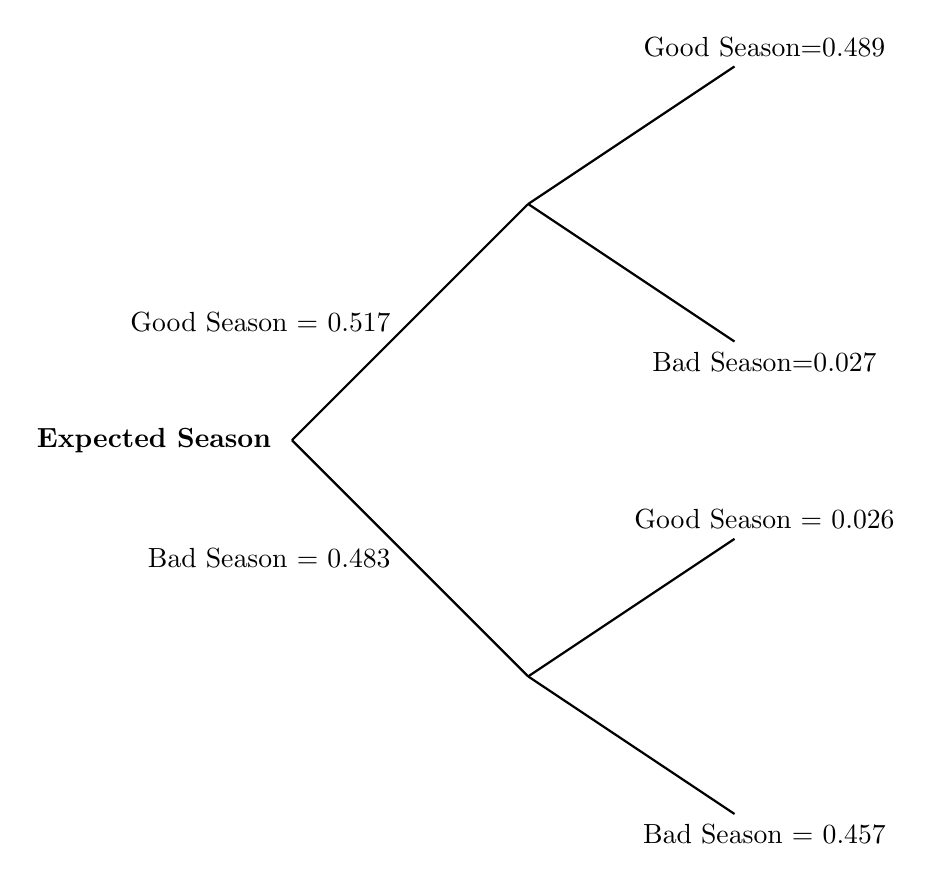
\begin{tikzpicture}[thick,
    level/.style={level distance=3cm},
    level 2/.style={sibling distance=6cm},
    level 3/.style={sibling distance=4cm}
]
\coordinate
child[grow=right, level distance=0pt] {
        child  {
            child {
                node {Bad Season = 0.457}
                edge from parent 
            }
            child {
                node {Good Season = 0.026}
                edge from parent
            }
            edge from parent
            node [left] {Bad Season = 0.483 \ }
        }
        child {
            child {
                node {Bad Season=0.027}
                edge from parent
            }
            child {
                node {Good Season=0.489}
                edge from parent  
            }
            edge from parent 
            node [left] {Good Season = 0.517 \ }
        }
        node [left] {\textbf{Expected Season\ \ }}
    };
\end{tikzpicture}
\end{figure}


\begin{figure}[htpb!]
\caption{Conception and Births: 40-45 Year-olds}
\hspace{8.0cm}\textbf{Realized Season} \vspace{4mm}\\
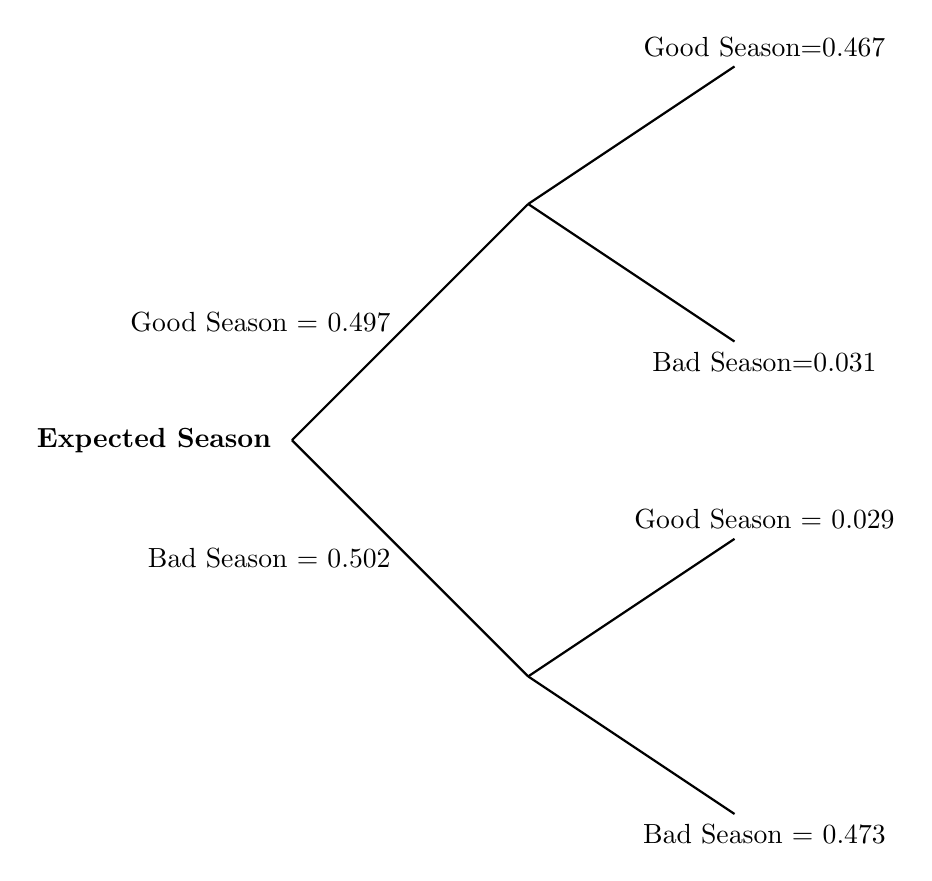
\begin{tikzpicture}[thick,
    level/.style={level distance=3cm},
    level 2/.style={sibling distance=6cm},
    level 3/.style={sibling distance=4cm}
]
\coordinate
child[grow=right, level distance=0pt] {
        child  {
            child {
                node {Bad Season = 0.473}
                edge from parent 
            }
            child {
                node {Good Season = 0.029}
                edge from parent
            }
            edge from parent
            node [left] {Bad Season = 0.502 \ }
        }
        child {
            child {
                node {Bad Season=0.031}
                edge from parent
            }
            child {
                node {Good Season=0.467}
                edge from parent  
            }
            edge from parent 
            node [left] {Good Season = 0.497 \ }
        }
        node [left] {\textbf{Expected Season\ \ }}
    };
\end{tikzpicture}
\end{figure}


\begin{figure}[htpb!]
\begin{center}
  \centering
  \caption{Good Season by State (Young)}
  \includegraphics[scale=0.34]{./../results/nvss/graphs/maps/young.png}
  \label{fig:mapYoung}
\end{center}
\end{figure}

\begin{figure}[htpb!]
\begin{center}
  \centering
  \caption{Good Season by State (Old)}
  \includegraphics[scale=0.34]{./../results/nvss/graphs/maps/old.png}
  \label{fig:mapOld}
\end{center}
\end{figure}

\begin{figure}[htpb!]
\begin{center}
  \centering
  \caption{Temperature and good Quarter: Young (Spain)}
  \includegraphics[scale=0.8]{./../results/spain/graphs/youngTempCold.eps}
  \label{fig:mapYoung}
\end{center}
\end{figure}
\clearpage

\begin{figure}[htpb!]
\begin{center}
  \centering
  \caption{Temperature and good Quarter: Old (Spain)}
  \includegraphics[scale=0.8]{./../results/spain/graphs/oldTempCold.eps}
  \label{fig:mapOld}
\end{center}
\end{figure}

\begin{figure}[htpb!]
\centering
\caption{Child quality: Birthweight (grams)}
\label{QBwt}
\includegraphics[scale=0.8]{../results/nvss/graphs/AllQuality_birthweight_.eps}
\end{figure}
\vspace{1cm}

\begin{figure}[htpb!]
\centering
\caption{Child quality: Birthweight (grams)}
\label{QApgar}
\includegraphics[scale=0.8]{../results/nvss/graphs/Quality_birthweight_.eps}
\end{figure}
\vspace{1cm}





\end{doublespace}
\end{document}



























\clearpage
\section{Data Appendix}
\label{bqScn:datApp}
\subsection{US Birth Data}
A brief description of US birth certificate data is provided in section
\ref{bqSscn:USAdata} of the paper.  As discussed, the format of US birth
certificates has undergone two important revisions: The first in 1989
and the second in 2003.  The date of adoption of these revisions varies
by state.  By 2013, 41 states or territories had adopted the revised (2003)
format, while the reaminder still follow the 1989 format.\footnote{The full
birth certificate for each revision is reproduced as figures 1 and 2 in
\citet{MenackerMartin2005}.  Over time the adoption of the 2003 certificate
was as follows: 2005: 12 (31\%), 2006: 19 (49\%), 2007: 22 (53\%), 2008: 27
(65\%), 2009: 28 (66\%), 2010: 33 (76\%), 2011: 36 (83\%), 2012: 38 (86\%),
and 2013: 41 (90\%).  In each case the first number refers to the number
of states, while the parenthesis indicates the percent of births in revised
states.}

In all cases where variable coding differs between the revised and unrevised
certificates (principally education for mother and father), we use the revised
2003 coding of the variables.  The reason we do this is because after 2008,
variables which are exclusive to 1989 certificates are no longer reported.
Figure \ref{bqFig:educMissing} illustrates this pattern.  The dotted line
represents the proportion of observations for maternal education which are
reported in the 1989 format, while the bars represent the proportion
\emph{missing} in the 2003 format.  From 2005-2008, all missing 2003 revision
variables are recorded in the 1989 format.  However, from 2009 onwards only
the 2003 revision of education is reported, meaning that those states who
still use the 1989 standard certificate do not have publicly released education
data.  %As expected, these are not missing at random, given that educational
%attainment varies considerably by state (see table \ref{bqTab:missingEduc}).
%In each case when these variables are used, we include full year and state
%fixed effects.




\begin{figure}[htpb!]
\caption{Missing Education Data by Time}
\label{bqFig:educMissing}
\includegraphics[scale=0.74]{../results/nvss/graphs/missingEduc.eps}
\end{figure}
%\input{./../results/nvss/regressions/NVSSMissingScale.tex}


\subsection{Spanish Data}

Birth certificate records from Spain are released by the National Institute of Statistics (INE)
with coverage from 1979 to 2013 inclusive. These consist of the universe of
births registered annually in Spain. Our principal estimation sample consists of
all first born children who survived one day, born to Spanish mothers. We use
births from the period 2007 to 2013, given that prior to 2007, education was not
recorded on birth certificates.  This results in a sample of 1,239,749 live
births, of which 1,238,685 were singletons.

Like birth certificate data in the US, Spanish certificates provide mother
and child characteristics, including education and labour market status of the
mother (and father where present), mother's age at time of birth, marital
status, and child APGAR, gestation, birth weight, prematurity, and so forth
\citep{INE2013}.  The Spanish records include publicly released data on
geographical location of birth, at both the provincial and municipal level
(similar to US states and counties respectively).

Descriptive statistics for Spanish births are provided in table \ref{bqTab:SumStatsSpain}.  In the same
age group, the average age and proportion of young mothers is similar to data
from USA (32 years and 96\% respectively), however a lower proportion report
being married (64\%), or having at least some post secondary education (53\%).
Spanish newborns are slightly lighter on average than their USA-born
counterparts (3,200g), however are also less likely to be born prematurely,
or classified as having low birth weight.

Spanish climate data at the level of the province is calculated from data released by the State Meteorological
Agency (AEMET). These data record the temperature at principal state
meteorological stations, from which we calculate monthly average, minima and
maxima.

\end{doublespace}
\end{document}
